\chapter{基于人类偏好对齐的检索增强对话生成}
\section{问题描述}

自LLM诞生以来,弥合人类意图和LLM之间的对齐差距一直是一个核心问题。在GPT-3\cite{DBLP:conf/nips/BrownMRSKDNSSAA20}时代,提示工程\cite{DBLP:conf/chi/ReynoldsM21},以及自动提示搜索\cite{DBLP:conf/emnlp/ShinRLWS20}和Prefix-Tuning\cite{DBLP:journals/corr/abs-2103-10385,lester-etal-2021-power,DBLP:conf/acl/LiL20},已经发展成为特定任务的校准者。然而,它们后来被指令微调\cite{DBLP:conf/iclr/WeiBZGYLDDL22}所取代和目前的RLHF方法\cite{DBLP:conf/nips/Ouyang0JAWMZASR22,DBLP:journals/corr/abs-2212-08073},将llm与人类偏好相结合,以训练llm将用户从繁重的提示中解放出来。

尽管如此,以训练为基础的结盟并不是唯一的解决方案。本质上,对齐差距可以从两个方向缩小:要么调整llm以接近人类偏好,要么改变人类提示以迎合llm的快速理解。例如,在图2中,展示了一个典型的用户提示——“告诉我关于哈利波特的事情”,这可能会导致一个简短的LLM响应。对于更详细和信息丰富的响应,虽然RLHF可以通过培训LLM来帮助实现相同的目标,但可以通过修改用户提示来实现相同的目标:“提供哈利波特系列的全面概述,包括书籍、电影、角色、主题和影响。在你的回答中要准确和翔实”。

更实际的是,随着llm变得越来越大,并且只能通过api访问,基于培训的对齐禁止小公司和个人开发人员按他们的意愿廉价和方便地对齐llm。相反,与从反馈方法中学习相比,偏好感知提示是有效的、非侵入的,并且更易于解释。因此,自动偏好感知提示是RLHF在LLM对齐中的一个有希望的补充,因此提出QAHF作为这个方向的第一个框架。

% 如上所述,我们的任务是优化用户输入,以帮助llm产生更好的响应。我们将用户输入表示为Xuser。我们的目标是构建一个函数F,将Xuser映射到它的优化版本,称为Xopt。为了实现这一点,引入了带注释的人类偏好,因为首选响应表明良好的模型输出,而另一个则表明较差的输出。通过捕获这些偏好数据之间的差异,可以将人类的偏好纳入用户指令中,使它们与llm可以做的事情更一致,从而使llm的输出更好地与人类的偏好一致。受最近利用llm作为评估者的工作启发(Wang等人,2023;郑等人,2023),我们认为llm具有理解不同响应中不同特征的能力。因此,我们选择利用llm来获得Xopt。具体来说,每个样本表示为(Xuser, Ygood, Ybad),其中Ygood表示有利响应,Ybad表示不利响应。因此,使用LLM的提示优化过程可以表示为Xopt = LLM(Xuser, Ygood, Ybad)。最后,我们通过在(Xuser, Xopt)对上训练一个较小的序列到序列模型来构建F函数。

\section{基于人类偏好对齐的检索增强对话生成}

\section{总体方案}

本章研究一种基于人类偏好对齐的检索增强对话生成的方法,该任务通常需要收集对话模型在各类真实场景下的对话,然后由人类完成偏好标注,最后通过PPO强化算法或其他算法训练对话模型,以达到偏好对齐的目的。而PPO强化学习在大型语言模型上非常具有挑战性,训练效果稳定性低。因此,本章提出基于人类反馈的问题对齐(Query Alignment with Human Feedback, QAHF)。如图\ref{qahf_framework}所示,QAHF方法主要包括四个阶段:1)人类偏好数据采集阶段;2)查询提示词构建阶段;3)查询有效性验证阶段;4)查询优化器训练阶段。

\begin{figure}[htbp]
	\centering
	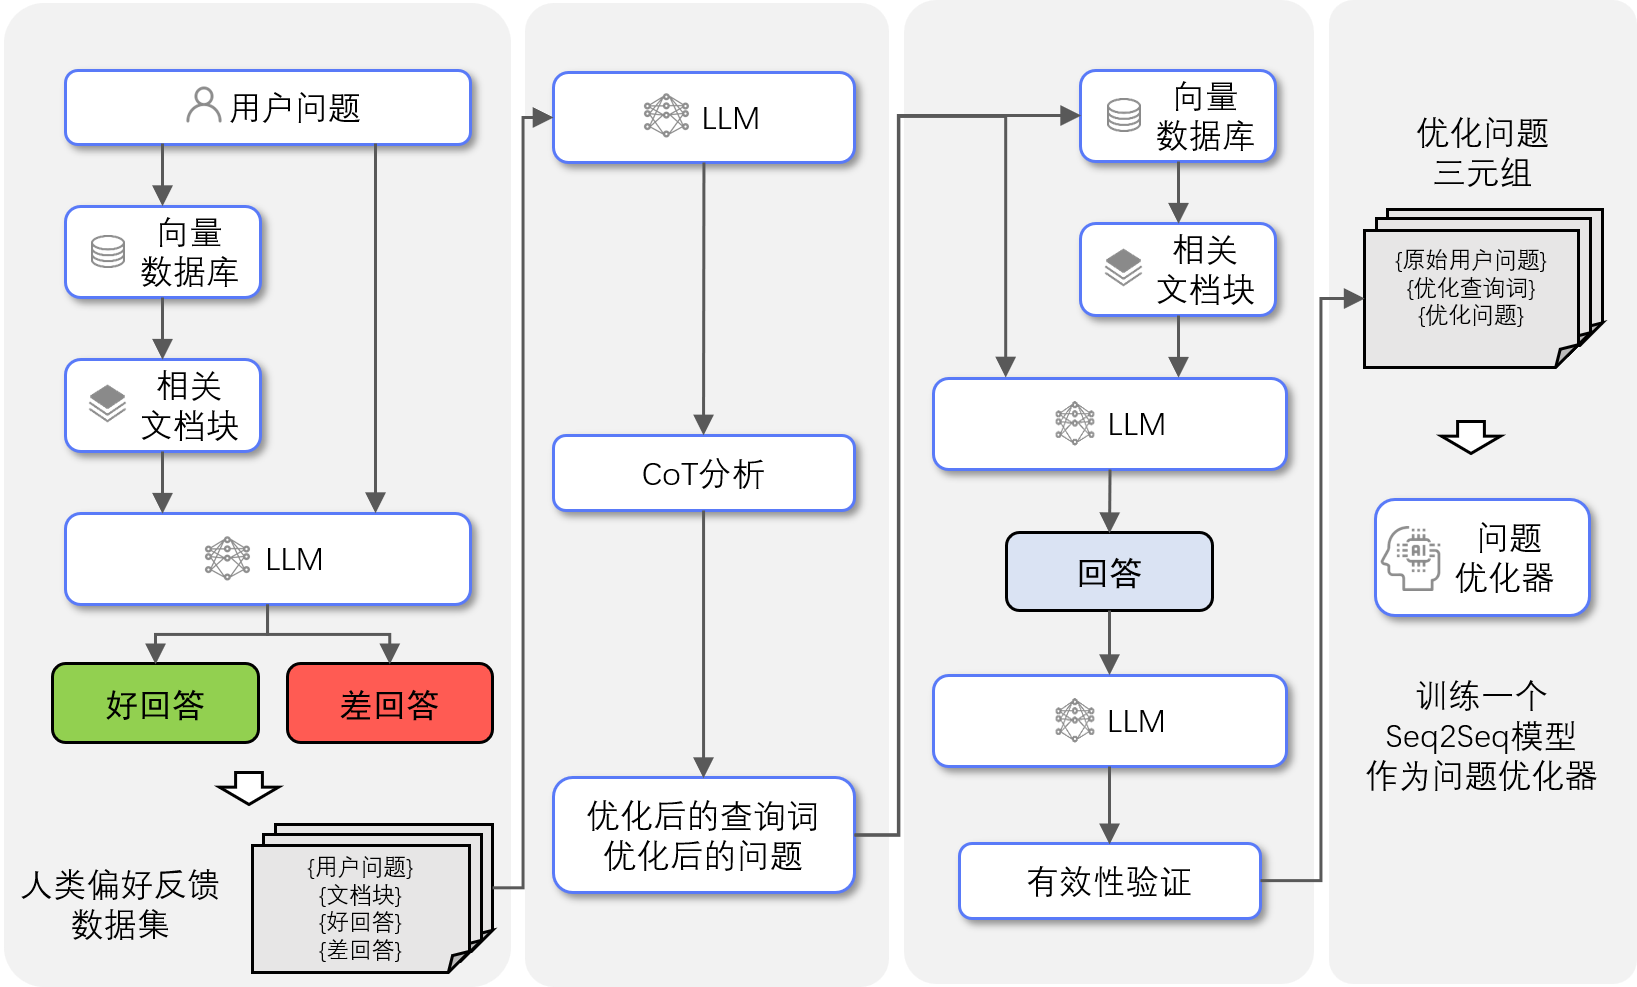
\includegraphics[scale=0.55]{Fig/qahf_framework.png}
	\caption{\label{qahf_framework}基于人类偏好对齐的检索增强对话生成框架图。}
\end{figure}

\subsection{人类偏好数据采集阶段}

为了建模人类偏好,本节首先搜集了一系列金融问答数据集,该数据集样本为“查询-回答”对,查询主题为金融相关专业问题。此外,本章使用基于规则的方法,过滤掉数据集中与金融领域无关、样本长度过短、查询范围过窄的低质量样本,以保证样本查询存在优化空间。然后,在向量数据库中检索与用户查询相关的文档块,并将结果输入LLM,通过随机采样的生成策略,得到LLM的多组回答。最后,通过人工标注的方式,从准确性、有帮助性、全面性等方面对LLM回答进行偏序关系标注,从每组回答中选出综合评分更高的回答作为“好回答”,评分最低的回答作为“差回答”,得到人类偏好反馈数据集。本章主要关注单轮对话的对话生成。

\subsection{优化查询构建阶段}

随后,本节使用LLM来对数据集中的原始用户查询进行优化。本节使用基于CoT的提示工程方法,引导LLM通过人类偏好反馈数据识别出用户偏好特征,分析造成LLM生成差回答的原因以及好回答中蕴含的人类偏好特征。接着,分别针对数据库检索和LLM对话场景各自生成一个优化后的查询语句,使得在新的查询语句下,检索增强对话系统生成的回答分布更趋近于好回答分布,区别于差回答的分布。本节所使用的查询优化提示词如表\ref{query_optimize_prompt}所示。

\begin{table}
	\caption{\label{query_optimize_prompt}查询优化提示词格式。}
	\centering{}%
	\small 
	\begin{tabular}{c}
		\toprule[2pt]
		查询优化提示词\tabularnewline
		\hline 
		\begin{tabular}{p{15cm}}
			\# SYSTEM\\你是一个大语言模型Prompt工程专家,你将根据我提供的信息完成我指定的任务。其中,QUERY表示用户输入的问题,DOCS是在数据库中检索得到的与QUERY相关的知识文档,GOOD RESPONSE是相比于BAD RESPONSE更符合人类偏好的LLM回复。 \\ \# QUERY \\ 作为个人知识答疑助手,请根据上述参考内容回答下面问题,答案中不允许包含编造内容。 \\ 问题是:<original query> \\ \# DOCS \\ <docs> \\ \# GOOD RESPONSE \\ <good response> \\ \# BAD RESPONSE \\ <bad response> \\ \# TASK \\ 你的任务是: \\ 1. 判断检索到的DOCS是否与QUERY相关,以及DOCS中的信息是否能够回答QUERY中的问题; \\ 2. 从事实性、完整性、逻辑性三个方面对比GOOD RESPONSE和BAD RESPONSE,分析可能导致LLM给出BAD RESPONSE的原因; \\ 3. 若DOCS与QUERY相关性不高,重写一个新的Query,用于数据库检索,使得检索到的DOCS的相关性更高,否则不需要重写; \\ 4. 作为专业的Prompt工程师,再重写一个新的QUERY,用于输入LLM,使得LLM更有可能给出GOOD RESPONSE。
		\end{tabular} \\
		\bottomrule[2pt]
	\end{tabular}
\end{table}

\subsection{查询有效性验证阶段}

LLM生成的问题可能仍然存在理解偏差问题,若直接使用带噪声的数据进行后续训练,可能加重模型理解偏差,损害模型性能。因此,本节将优化后的问题重新输入系统,得到新的模型回复,并利用大型语言模型的反思能力,对新回复的质量进行评判,以筛选出有效的偏好数据样本,提高数据集信噪比。并得到最终的优化问题三元组数据集。其中,本阶段所使用的查询有效性验证提示词如表\ref{query_validation_prompt}所示。
% TODO:包含三步骤...

\begin{table}
	\caption{\label{query_validation_prompt}查询有效性验证提示词格式}
	\centering{}%
	\small 
	\begin{tabular}{c}
		\toprule[2pt]
		有效性验证提示词\tabularnewline
		\hline 
		\begin{tabular}{p{15cm}}
			\#SYSTEM \\ 你是一个大语言模型Prompt工程专家,你将根据我提供的信息完成我指定的任务。其中,QUERY表示用户输入的问题,DOCS是在数据库中检索得到的与QUERY相关的知识文档,RESPONSE是LLM的回复。 \\ \# QUERY \\ 作为个人知识答疑助手,请根据上述参考内容回答下面问题,答案中不允许包含编造内容。 \\ 问题是:<original query> \\ \# DOCS \\ <docs> \\ \# RESPONSE \\ < response> \\ \# TASK \\ 你的任务是: \\ 1. 判断检索到的DOCS是否与QUERY相关,以及DOCS中的信息是否能够回答QUERY中的问题; \\ 2. 判断RESPONSE是否能够准确、可靠地回答QUERY; \\ 3. 对RESPONSE进行评分,分数取值范围为[1, 10]。 \\ 
		\end{tabular} \\
		\bottomrule[2pt]
	\end{tabular}
\end{table}

\subsection{查询优化器训练阶段}

基于前述步骤所构建的人类偏好数据集,训练一个Seq2Seq模型作为查询优化器,实现模型无关的、可插拔的用户查询自动优化。形式上,给定原始用户查询$Q_{ori}$,优化器生成优化后的查询$Q_{opt}$:
\begin{equation}
	Q_{opt} = [Q_{search}, [SEP], Q_{qa}]
\end{equation}
其中,$Q_{search}$表示用于数据库检索的查询,$Q_{qa}$表示用于回答生成的查询,$[SEP]$为特殊字符,用于分隔$Q_{search}$和$Q_{qa}$。

本节使用交叉熵损失函数作为训练目标,损失函数定义为:
\begin{equation}
	L=-\frac{1}{N} \sum_{t=1}^N \log P\left(x_t \mid Q_{\text{ori}}, x_{<t}\right)
\end{equation}
其中,$N$是$Q_{opt}$的长度,$x_t$表示$Q_{opt}$中的第$t$个字符。本章选择Qwen-7B作为基座模型,以更好地学习$Q_{ori}$和$Q_{opt}$之间的隐式偏好映射。同时,在目前的主流LLM中,7B模型的参数量相对较小,能够以更低的成本进行训练和推理,具有更低的推理延迟,作为本方法中的查询优化器具有一定优势。

\section{实验}

\subsection{数据集介绍}

FinGPT-FiQA\cite{wang2023fingptbenchmark}是Wang等人创建的人工评估数据集。它包含了17.1k个金融领域的用户查询与回答样本,这些样本均采样于真实应用场景。本节从中抽取了1000条样本作为实验的测试数据。

AlphaFin-test是本文第三章中构建的数据集的一部分,它包含1000条问答数据对,数据集从StockQA和research数据集中采样。AlphaFin-test数据集能够评估模型在资本市场上的能力。

\subsection{评价指标}

本节使用人类和GPT4模型作为评判员,对两种不同模型或不同方法的生成结果进行两两对比,以更好地评估不同方法之间性能差异。另外,本节还采用Ragas\cite{DBLP:conf/eacl/ESJAS24}指标自动化评估模型回复的质量。本节所使用的ragas评价指标包括:(1)Context Precision;(2)Context Recall;(3)Faithfulness。

\subsection{基础模型与基准方法}

基础模型:

Qwen-7B-Chat\cite{qwen}:通义千问-7B(Qwen-7B)是阿里云研发的通义千问大模型系列的70亿参数规模的模型。Qwen-7B是基于Transformer的大语言模型, 在超大规模的预训练数据上进行训练得到。预训练数据类型多样,覆盖广泛,包括大量网络文本、专业书籍、代码等。

FinGPT\cite{yang2023fingpt}:FinGPT 是2023年6月哥伦比亚大学联合上海纽约大学推出全新大模型产品,这是一款面向金融领域的大模型产品。它使用自建金融数据集在llama2-13b、ChatGLM2-6B等预训练模型上进行LoRA微调,得到金融领域语言模型。本实验所使用的是基于ChatGLM2-6B的版本。

ChatGLM2-6B\cite{DBLP:conf/iclr/ZengLDWL0YXZXTM23}:ChatGLM2-6B是智谱AI及清华KEG实验室发布的中英双语对话模型。它使用了 GLM 的混合目标函数,经过了 1.4T 中英标识符的预训练与人类偏好对齐训练,在CEval、GSM8K等数据集上得到大幅度的性能提升。同时,ChatGLM2-6B使用了 Multi-Query Attention,提高了生成速度,同时也降低了生成过程中 KV Cache 的显存占用。同时,ChatGLM2-6B 采用 Causal Mask 进行对话训练,连续对话时可复用前面轮次的 KV Cache,进一步优化了显存占用。

ChatGPT\cite{DBLP:conf/nips/Ouyang0JAWMZASR22}:ChatGPT全名Chat Generative Pre-trained Transformer,是由OpenAI开发的一款基于人工智能技术的聊天机器人程序,于2022年11月30日发布。它基于GPT(Generative Pre-trained Transformer)架构,这是一种自然语言处理(NLP)模型,能够理解和生成人类的自然语言。

基准方法:

PPO\cite{DBLP:journals/corr/SchulmanWDRK17}:PPO算法是在Policy Gradient算法的基础上由来的,Policy Gradient是一种on-policy的方法,他首先要利用现有策略和环境互动,产生学习资料,然后利用产生的资料,按照Policy Gradient的方法更新策略参数。然后再用新的策略去交互、更新、交互、更新,如此重复。

BPO\cite{DBLP:journals/corr/abs-2311-04155}:黑盒提示优化(Black-Box Prompt Optimization,BPO)算法,自动优化用户输入,以更好地适应llm对改进响应的偏好。通过BPO对齐,无需进一步微调对话模型,即可对齐人类和模型之间的理解偏差。但本方法仅使用用户问题和模型回复构建偏序数据集,在检索增强应用场景下,没有考虑检索的知识文档信息,因此还有很大的空间可以进一步提升。

\subsection{实现细节}

对于QAHF,本节使用Qwen-7B作为优化器基座模型,在所构建的问题优化三元组数据集上对优化器模型训练了3个epoch。只需要保存最后一个checkpoint。在训练阶段,本节使用AdamW优化器,$\beta1$=0.9和$\beta2$=0.999。本实验将学习率设置为2e-5,热启动步长为0.1\%,使用线性衰减学习率。每个GPU的batch size大小为4。对于RLHF训练,RM模型训练和PPO优化只训练1个epoch。其中,本实验RM模型的训练数据来自于本章方法所构建的人类偏好数据集,RM模型在同分布测试集上达到了78\%的准确率。所有实验均在8×80GB NVIDIA A800 GPU上进行。QAHF采用Top-p=0.9和Temperature=0.6进行推理解码,而所有测试的基座模型都使用默认的解码策略。

\subsection{与现有方法的性能比较}

\begin{table}
	\caption{\label{qahf_single_performance}QAHF在FinGPT-FiQA Eval和AlphaFin-test上的有效性实验}
	\centering
	\begin{tabular}{lcc|ccc|ccc|c}
		\toprule[2pt]
		\multirow{2}*{模型} & \multicolumn{2}{c|}{方法} & \multicolumn{3}{c|}{FinGPT-FiQA Eval} & \multicolumn{3}{c|}{AlphaFin-test} & \multirow{2}*{$\Delta$ WR} \\
		\cline{2-9}
		~ & A & B & A win & Tie & B win & A win & Tie & B win & ~ \\
		\hline
		ChatGLM & QAHF & ori. & 58.0\% & 21.0\% & 21.0\% & 61.0\% & 5.2\% & 33.8\% & +32.1\% \\
		FinGPT & QAHF & ori. & 57.5\% & 22.4\% & 20.1\% & 54.3\% & 15.1\% & 30.6\% & +30.5\% \\
		Qwen & QAHF & ori. & 52.2\% & 15.5\% & 32.3\% & 54.0\% & 12.3\% & 33.7\% & +20.1\% \\
		ChatGPT & QAHF & ori. & 39.0\% & 26.3\% & 34.7\% & 41.1\% & 27.1\% & 31.8\% & +6.8\% \\
		\bottomrule[2pt]
	\end{tabular}
\end{table}

详细的实验结果如表\ref{qahf_single_performance}所示。基于本章所提出的QAHF方法,在所有基座模型和所有数据集上,其性能均优于原始查询,取得了更高的胜率,证明了本章方法的有效性和广泛适用性。值得注意的是,在ChatGLM、FinGPT、Qwen等相对小尺寸的开源模型上,QAHF相比于原始查询的胜率分别提高了32.1\%、30.5\%和20.1\%,FinGPT在数据集FinGPT-FiQA Eval上甚至达到了37.4\%的提升,而在gpt-3.5-turbo这类模型上,胜率提升在10\%以内,说明本章方法对于尺寸更小、基础能力相对更弱的基座模型能够收获更大的对齐收益。

\begin{table}
	\caption{\label{qahf_bpo_performance}QAHF与BPO在FinGPT-FiQA Eval和AlphaFin-test上的性能对比}
	\centering
	\begin{tabular}{lcc|ccc|ccc|c}
		\toprule[2pt]
		\multirow{2}*{模型} & \multicolumn{2}{c|}{方法} & \multicolumn{3}{c|}{FinGPT-FiQA Eval} & \multicolumn{3}{c|}{AlphaFin-test} & \multirow{2}*{$\Delta$ WR} \\
		\cline{2-9}
		~ & A & B & A win & Tie & B win & A win & Tie & B win & ~ \\
		\hline
		\multirow{3}*{ChatGLM} & BPO & ori. & 43.2\% & 22.4\% & 34.4\% & 40.7\% & 15.6\% & 43.7\% & +3.0\% \\
		~ & QAHF & BPO & 36.8\% & 39.6\% & 23.6\% & 52.5\% & 12.7\% & 34.8\% & +15.4\% \\
		~ & QAHF & ori. & 58.0\% & 21.0\% & 21.0\% & 61.0\% & 5.2\% & 33.8\% & +32.1\% \\
		\hline
		\multirow{3}*{ChatGPT} & BPO & ori. & 39.4\% & 12.3\% & 48.3\% & 43.6\% & 25.5\% & 30.9\% & +1.9\% \\
		~ & QAHF & BPO & 31.1\% & 38.5\% & 30.4\% & 40.9\% & 28.2\% & 30.9\% & +5.4\% \\
		~ & QAHF & ori. & 39.0\% & 26.3\% & 34.7\% & 41.1\% & 27.1\% & 31.8\% & +6.8\% \\
		\bottomrule[2pt]
	\end{tabular}
\end{table}

如表\ref{qahf_bpo_performance}所示,BPO和QAHF均成功提升了ChatGLM和gpt-3.5-turbo模型的性能。此外,在QAHF与BPO的所有对比实验中,QAHF均取得了正向的胜率提升,近一步证明QAHF方法相较于BPO方法的优越性。

\begin{table}
	\caption{\label{qahf_ppo_performance}QAHF与PPO在FinGPT-FiQA Eval和AlphaFin-test上的性能对比}
	\centering
	\begin{tabular}{lcc|ccc|c}
		\toprule[2pt]
		\multirow{2}*{模型} & \multicolumn{2}{c|}{方法} & \multicolumn{3}{c|}{AlphaFin-test} & \multirow{2}*{$\Delta$ WR} \\
		\cline{2-6}
		~ & A & B & A win & Tie & B win & ~ \\
		\hline
		\multirow{3}*{ChatGLM} & PPO & ori. & 13.7\% & 75.4\% & 10.9\% & +2.8\% \\
		~ & QAHF & PPO & 49.3\% & 20.6\% & 30.1\% & +19.2\% \\
		~ & QAHF & ori. & 61.0\% & 5.2\% & 33.8\% & +27.2\% \\
		\bottomrule[2pt]
	\end{tabular}
\end{table}

同时,本实验还对比了QAHF和PPO强化学习对齐方法的性能差异,结果如表\ref{qahf_ppo_performance}所示。从表中可以看出,由于PPO训练稳定性较差,虽然训练实现了收敛,但PPO方法对模型性能的提升较为有限,75.4\%的样本没有明显提升,胜率仅有2.8\%。而QAHF方法依然能获得10\%以上的稳定提升。

\begin{table}
	\caption{\label{query_compare_sota}使用不同对齐方法优化后的用户问题对比}
	\centering
	\begin{tabular}{cc}
		\toprule[2pt]
		类型 & 问题 \\
		\hline
		原始 & \begin{tabular}{p{12cm}}
			招商证券2020年下半年市场份额如何?
		\end{tabular} \\
		\hline
		BPO & \begin{tabular}{p{12cm}}
			招商证券2020年下半年在代理买卖证券业务、股权投资收益、财富管理等方面的表现如何?
		\end{tabular} \\
		\hline
		\begin{tabular}{c}
			QAHF \\ (本章方法)
		\end{tabular} & \begin{tabular}{p{12cm}}
			根据招商证券2020年下半年的业务增长情况和市场排名,描述该公司在市场份额方面的表现。
		\end{tabular} \\
		\bottomrule[2pt]
	\end{tabular}
\end{table}

本节对比原始用户问题和使用BPO、QAHF方法进行优化后的问题,得到结果如表\ref{query_compare_sota}所示。从表中可以看出,BPO方法没有考虑检索得到的知识文档信息,而直接对用户问题和模型回复进行分析和重写,因此重写后的问题局限于参考回答中的局部信息,而QAHF方法根据检索到的研报和新闻数据,分析出文档包含了该公司的市场份额相关信息,包括各项业务的增长情况、市场排名等,因此将原始用户问题中的表述扩展为“业务增长情况和市场排名”。

\begin{table}
	\caption{\label{response_compare_sota}使用不同对齐方法优化用户查询后得到的模型回复对比}
	\centering
	\begin{tabular}{cc}
		\toprule[2pt]
		类型 & 回复 \\
		\hline
		原始 & \begin{tabular}{p{12.5cm}}
			抱歉,根据上述参考内容,我们无法得出关于招商证券2020年下半年市场份额的具体信息,因为该报告只提到了公司在2020年全年的业绩和排名情况,而没有涉及到下半年市场的份额变化。同时,该报告也没有提供关于个人知识答疑助手日期和招商证券2020年下半年市场份额的任何信息。
		\end{tabular} \\
		\hline
		BPO & \begin{tabular}{p{12.5cm}}
			从提供的研报中可以得知,招商证券在2020年下半年表现出了良好的增长态势。具体来说,公司各项业务全面增长,其中经纪业务增速最高,实现营收67.2亿元,同比37.1\%;自营业务规模也有提升,营收同比增长10.1\%。公司在投资银行业务方面表现较为突出,投行业务收入同比增长18.4\%,但股权投资收益同比仅略微下降。此外,公司的代理买卖证券业务也有所提升,但两项业务的市场份额排名均有所下降。因此,可以预测,招商证券在2020年下半年将继续保持良好的增长势头,但需要关注市场波动和业务风险。
		\end{tabular} \\
		\hline
		\begin{tabular}{c}
			QAHF \\ (本章 \\ 方法)
		\end{tabular} & \begin{tabular}{p{12.5cm}}
			作为知识答疑助手,我认为招商证券2020年下半年市场份额如下: \\ 排名提升:在2020年上半年,招商证券的股票托管业务和股票经纪业务分别排名第6和第8位,但是在下半年,这两个业务的排名都提升了,分别排名第2和第3位。 \\ 市场份额上升:在2020年下半年,招商证券的代理业务同比增长了26\%,达到了2294.27亿元,占公司总代理业务收入的41.94\%,而2019年同期仅占2719.3亿元,占公司总代理业务收入的11.93\%。 \\ 头部地位稳固:在2020年下半年,招商证券的经纪业务、投行和资管业务分别排名第1、第7和第2位,而公司总代理业务排名第3位,这表明公司在行业中的地位稳固,继续保持头部地位。 \\ 因此,从2020年下半年招商证券的市场份额来看,在提升了代理业务的市场份额下,公司经纪业务、投行和资管业务仍保持了头部地位,并且在提高市场份额的同时,公司的代理业务同比增长了26\%。
		\end{tabular} \\
		\bottomrule[2pt]
	\end{tabular}
\end{table}

基于上述三种原始问题和优化问题,得到的模型回复情况如表\ref{response_compare_sota}所示。从表中可以看出,基于原始问题,模型无法准确理解市场份额的意义,因此认为知识文档中不包含与此相关的内容,做出了拒绝回答的行为;基于BPO优化后的问题聚焦于更细分的代理买卖证券业务、股权投资收益、财富管理等方面,但由于与知识文档内容存在偏差,模型回复出现编造数据等偏离事实性的现象;基于QAHF优化后的问题,紧扣知识文档内容,同时对简单的问题进行详细展开,使得模型能更好抓住文档中的重点,因此回复更详细且数据准确。

\subsection{查询有效性验证模块的有效性}

QAHF的一个重要组成部分是利用反馈来优化用户指令。为了研究反馈对QAHF的快速优化有多大贡献,进行了消融实验,以比较反馈学习优化(QAHF)和直接使用gpt-3.5-turbo进行快速优化。如表\ref{evaluation_pk_fiqa}和表\ref{evaluation_pk_alphafin}所示,直接优化可以提高模型性能,这验证了llm成为良好提示工程师的潜力。QAHF提供了超越直接优化的进一步改进。这表明,纳入反馈允许llm根据所展示的用户偏好来完善提示,从而实现更有效的提示优化。

\begin{table}
	\caption{\label{evaluation_pk_fiqa}在FinGPT-FiQA数据集上探究查询有效性验证模块对性能的影响}
	\centering
	\begin{tabular}{lcc|ccc|c}
		\toprule[2pt]
		\multirow{2}*{模型} & \multicolumn{2}{c|}{方法} & \multicolumn{3}{c|}{FinGPT-FiQA Eval} & \multirow{2}*{$\Delta$ WR} \\
		\cline{2-6}
		~ & A & B & A win & Tie & B win & ~ \\
		\hline
		\multirow{3}*{ChatGLM} & QAHF & ori. & 58.0\% & 21.0\% & 21.0\% & +32.1\% \\
		~ & w/o Eval & ori. & 49.8\% & 25.5\% & 24.7\% & +24.8\% \\
		~ & QAHF & w/o Eval & 8.6\% & 86.3\% & 5.1\% & +4.5\% \\
		\bottomrule[2pt]
	\end{tabular}
\end{table}


\begin{table}
	\caption{\label{evaluation_pk_alphafin}在AlphaFin-test数据集上探究查询有效性验证模块对性能的影响}
	\centering
	\begin{tabular}{lcc|ccc|c}
		\toprule[2pt]
		\multirow{2}*{模型} & \multicolumn{2}{c|}{方法} & \multicolumn{3}{c|}{AlphaFin-test} & \multirow{2}*{$\Delta$ WR} \\
		\cline{2-6}
		~ & A & B & A win & Tie & B win & ~ \\
		\hline
		\multirow{3}*{ChatGLM} & QAHF & ori. & 61.0\% & 5.2\% & 33.8\% & +32.1\% \\
		~ & w/o Eval & ori. & 46.9\% & 30.6\% & 22.5\% & +24.8\% \\
		~ & QAHF & w/o Eval & 15.1\% & 75.3\% & 9.6\% & +4.5\% \\
		\bottomrule[2pt]
	\end{tabular}
\end{table}

本节基于ragas评估框架对完整的QAHF方法和去除提示词有效性验证模块后的QAHF方法进行性能比较,实验结果如表\ref{evaluation_ragas}所示。从表中结果可以看出,去除提示词有效性验证模块后,数据中噪声偏多,因此模型在context\_precision和faithfulness指标上都仅有0.03和0.02的微弱提升,甚至在context\_recall上有0.01的降低。而增加提示词有效性验证模块后,模型在context\_precision和faithfulness指标上有了显著提升,分别提升了0.11和0.06分,而在context\_recall指标上,与原始结果几乎相同,仅相差0.001。对于context\_recall指标上分数的降低,可能是因为问题改写仅影响模型回复与用户问题之间的相关性,而context\_recall评估的是用户问题和知识文档之间的相似性,因此在这一指标上,所对比的三种方法得分相近。

\begin{table}
	\caption{\label{evaluation_ragas}在Ragas指标上查询有效性验证模块对性能的影响}
	\centering
	\begin{tabular}{c|cccc}
		\toprule[2pt]
		模型 & 方法 & Precision $\uparrow$ & Recall $\uparrow$ & Faithfulness $\uparrow$ \\
		\hline
		\multirow{3}*{ChatGLM} & ori. & 0.6717 & 0.8430 & 0.8005 \\
		~ & w/o Eval & 0.7023(+0.03) & 0.8329(-0.01) & 0.8216(+0.02) \\
		~ & QAHF & 0.7839(+0.11) & 0.8417(-0.001) & 0.8574(+0.06) \\
		\bottomrule[2pt]
	\end{tabular}
\end{table}

同时,表\ref{valid_invalid_example}展示了具体的有效样本和无效样本内容,从示例内容可以看出,无效样本的优化问题将原始问题中的“杭州公司股票”改为了“杭州的公司”,导致问题对象发生变化,导致最终模型回复不符合用户初始意图。有效性验证模块能够准确地从初始数据集中过滤无效样本,提高训练数据集的信噪比,避免进一步加重模型的幻觉现象。

\begin{table}
	\caption{\label{valid_invalid_example}有效样本与无效样本对比}
	\centering
	\begin{tabular}{c|c|c}
		\toprule[2pt]
		\multicolumn{2}{c|}{类型} & 内容 \\
		\hline
		\multirowcell{3}{有效\\样本} & 原始问题 & \begin{tabular}{p{11.7cm}}
			国庆黄金周对旅游股有什么影响
		\end{tabular} \\
		\cline{2-3}
		~ & 优化问题 & \begin{tabular}{p{11.7cm}}
			国庆黄金周对旅游股有什么影响,列点回答,从宏观到微观依次分析对旅游行业、旅游公司、旅游股的影响,最后给出综合性结论。
		\end{tabular} \\
		\cline{2-3}
		~ & 模型回复 & \begin{tabular}{p{11.7cm}}
			国庆黄金周对旅游股的影响主要体现在以下几个方面:\\1.客流量增加:…\\2.板块内部分红机会:…\\3.旅游股的业绩弹性:…\\4.旅游股面临了一定的市场风险:…\\综上所述,国庆黄金周对旅游股的影响主要体现在客流量增加、板块内部分红机会、旅游股的业绩弹性和面临的市场风险等方面。投资者在关注国庆黄金周带来的投资机会的同时,还需注意国庆期间的市场风险,合理制定投资策略。
		\end{tabular} \\
		\hline
		\multirowcell{3}{无效\\样本} & 原始问题 & \begin{tabular}{p{11.7cm}}
			杭州亚运会对杭州公司股票有什么积极作用
		\end{tabular} \\
		\cline{2-3}
		~ & 优化问题 & \begin{tabular}{p{11.7cm}}
			杭州亚运会对杭州的公司有什么积极作用
		\end{tabular} \\
		\cline{2-3}
		~ & 模型回复 & \begin{tabular}{p{11.7cm}}
			杭州亚运会将为杭州的公司带来积极影响,具体来说:\\1.亚运会将带来大量游客:…\\2.亚运会将带动周边房价上涨:…\\3.亚运会将推动杭州文化产业发展:…\\4.亚运会将带动杭州基础设施建设:…\\总之,杭州亚运会将为杭州的公司带来诸多积极影响,包括游客、房价、文化产业和基础设施等方面。这些都将为杭州的公司提供更多的商业机会和发展动力。
		\end{tabular} \\
		\bottomrule[2pt]
	\end{tabular}
\end{table}

\subsection{迭代优化对算法性能的影响}

由于QAHF可以优化用户提示以获得更好的响应,自然的想法是是否可以迭代优化问题,逐步增强LLM的输出。因此,本节用gpt-3.5-turbo在AlphaFin-test数据集上进行了实验。具体来说,本节对原始指令进行了5次迭代优化,并与原始指令进行了ragas指标比较。如图\ref{multi_iter_optimize_ragas_exp}所示,通过3次迭代,有明显的改善,在第4次迭代时略有下降。此外,本节还发现QAHF表现出良好的保留性,当输入提示已经足够好时,它有很高的概率保留它。本节认为这是实现迭代增强的关键因素,因为它避免了对用户的原始意图进行不合理的更改。多次执行CoT分析与优化问题生成。

\begin{figure}[htbp]
	\centering
	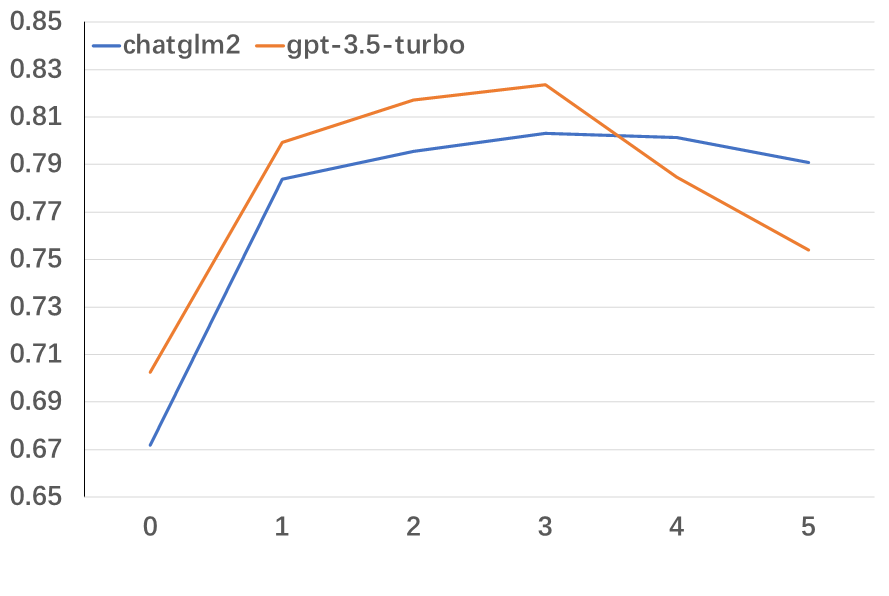
\includegraphics[scale=0.5]{Fig/multi_iter_optimize_ragas_exp.png}
	\caption{\label{multi_iter_optimize_ragas_exp}经过不同迭代优化次数的Ragas Precision变化示意图。}
\end{figure}

\subsection{人类反馈对算法性能的影响}

QAHF的一个重要组成部分是利用反馈来优化用户指令。为了研究反馈对QAHF的快速优化有多大贡献,进行了消融实验,以比较反馈学习优化(QAHF)和直接使用gpt-3.5-turbo进行快速优化。如表\ref{human_feedback_pk}所示,直接优化可以提高模型性能,这验证了llm成为良好提示工程师的潜力。QAHF提供了超越直接优化的进一步改进。这表明,纳入反馈允许llm根据所展示的用户偏好来完善提示,从而实现更有效的提示优化。

\begin{table}
	\caption{\label{human_feedback_pk}在偏好评价指标上人类反馈对性能的影响}
	\centering
	\begin{tabular}{lcc|ccc|c}
		\toprule[2pt]
		\multirow{2}*{模型} & \multicolumn{2}{c|}{方法} & \multicolumn{3}{c|}{AlphaFin-test} & \multirow{2}*{$\Delta$ WR} \\
		\cline{2-6}
		~ & A & B & A win & Tie & B win & ~ \\
		\hline
		\multirow{3}*{ChatGLM} & QAHF & ori. & 61.0\% & 5.2\% & 33.8\% & +27.2\% \\
		~ & w/o Human & ori. & 39.4\% & 35.8\% & 24.8\% & +14.6\% \\
		~ & QAHF & w/o Human & 45.7\% & 20.3\% & 34.0\% & +11.7\% \\
		\bottomrule[2pt]
	\end{tabular}
\end{table}

\section{本章小结}

本章提出基于人类偏好对齐的检索增强对话生成方法,能够实现与模型无关的、可解释、效果稳定的人类偏好对齐。此外,本章提出的人类偏好对齐方法还面临着受限于标注者的主观偏好的问题,因此在未来的工作中,这也是需要进一步研究和完善的方向。